\chapter{Reddit-Based Sentiment Analysis}
\label{chap:sentiment_reddit}

\begin{introduction}
This appendix describes the pipeline used to derive sector-specific sentiment labels from Reddit threads. An ensemble of three large language models first annotates a representative subset of the data to produce a labelled dataset, which is subsequently augmented, and a lightweight ModernBERT-based classifier is then trained on the augmented dataset and applied to the full Reddit corpus to generate the sentiment features used in the main analysis.
\end{introduction}

Unlike GDELT quotes, which were pre-filtered by sector prior to annotation, Reddit threads have no inherent sector association. The annotation task therefore requires the model to assess, for each post, whether and how its content relates to each of the 11 GICS sectors. This multi-label framing adds considerable complexity: a single thread discussing broad macroeconomic conditions, for instance, may simultaneously carry positive implications for Financials, negative ones for Real Estate, and remain irrelevant to Consumer Staples.

To manage this complexity, a two-stage pipeline is applied. In the first stage, an LLM ensemble annotates a representative sample of Reddit threads, producing sector-level sentiment labels across all 11 sectors. In the second stage, a dedicated classifier is trained on this labelled dataset and used to score the full corpus at scale.

\section{LLM-Based Annotation}
\label{sec:redditllm_annotation}

Since Reddit posts carry no prior sector association, the LLM ensemble must evaluate each post against all 11 GICS sectors simultaneously. This is a more demanding annotation task than the GDELT case, as the model must assess relevance and sentiment direction for each sector independently, often in the absence of explicit sector mentions.

Three LLMs are used: \texttt{meta-llama/Llama-3.1-8B-Instruct}, \texttt{google/gemma-7b-it}, and \texttt{Qwen/Qwen2.5-7B-Instruct}. They are used as annotators, each receiving the same structured prompt. For each sector, the final label is determined by majority vote across the three models. A sample of $\num{19019}$ threads were labeled from the full corpus of $\num{355352}$ Reddit threads, requiring approximately $\num{950}$ GPU-hours on a dual NVIDIA T4 setup. 

\subsection{Prompt Design and Thread Representation}
\label{sec:redditprompt}

The prompt, shown in Fig.~\ref{fig:redditprompt}, was designed to elicit a single structured JSON response covering all 11 sectors at once. It defines what constitutes a meaningful sentiment signal, as opposed to a casual mention or unsubstantiated opinion, and specifies \textit{neutral} as the default label when sector relevance is unclear. At inference time, the post's title, body, and top comments were concatenated to reconstruct the discussion thread, which was injected into the prompt as \texttt{<THREAD>}.

The \texttt{<THREAD>} representation, for both annotation and later classification, includes the post's title and body, followed by the most upvoted comments. Top comments are prioritized because they tend to contain the most substantive discussion and sentiment signals, as opposed to the long tail of less visible replies. To manage input length and keep the model focused on the most relevant content, comment accumulation is capped once both a minimum of $\num{10}$ comments and $\num{1000}$ characters of comment text have been collected, or when the thread's comment list is exhausted, whichever comes first. This approach balances the need to capture meaningful discussion with the practical constraints of model input limits and inference cost.

% moved fig fig:redditprompt to the next section

\subsection{Vote Distribution}
\label{sec:redditvote_distribution}

Table~\ref{tab:redditsentiment_votes_sector} reports the distribution of sentiment labels across sectors, broken down by the number of LLMs that agreed on the assigned label (1, 2, or 3 votes). The class \textit{neutral} dominates across all sectors, which is expected: most Reddit threads do not contain substantive, directional commentary on any given sector, and the prompt's conservative definition of a meaningful sentiment signal actively discourages spurious positive or negative labels.

The distribution of 3-vote consensus varies considerably across sectors. Sectors such as Consumer Staples, Utilities, and Real Estate show very high neutral consensus and very few clear positive or negative signals, reflecting their relative scarcity in retail investor discussion. By contrast, Information Technology, Consumer Discretionary, and Financials attract more varied and opinionated content, yielding a wider spread of non-neutral labels and higher disagreement rates, consistent with real-world observations that these sectors dominate retail trading discussion.

% belongs to the previous section, but moved here
\begin{figure}[H]
\centering
\begin{tcolorbox}
\ttfamily\small
You are a financial-domain sentiment classifier specializing in equity markets.

Your task is to analyze Reddit stock discussion threads and assign a sentiment label — "positive", "neutral", or "negative" — to each of the 11 official GICS sectors based on how the thread discusses companies, industries, events, or themes related to each sector.

$\ $

Classification Rules:

- "positive": applies only if the thread expresses MEANINGFUL bullishness, optimism, expected gains, or favorable news for a sector.

- "negative": applies only if the thread expresses MEANINGFUL bearishness, pessimism, expected declines, or harmful news for a sector.

- "neutral": applies when the thread does not meaningfully reference the sector, sentiment is unclear, or discussion is casual/speculative without substance; default sentiment.

$\ $

A reference is meaningful only if it includes at least one of the following:

- A clear expectation of price movement or performance (up or down)

- A stated reason, catalyst, or justification (e.g., earnings, news, macro factors, valuation)

- Repeated or emphasized sentiment across multiple comments

- Explicit long or short positioning with intent

$\ $

The following are NOT meaningful by themselves:

- Casual mentions of company names

- Jokes, memes, sarcasm, or one-line opinions

- Watchlists, tickers without commentary, or gap lists

- Statements without reasoning (e.g., "this stock will moon" or "short it" without explanation)

\begin{verbatim}
Output Requirements:
Return your response strictly as a JSON object with the following fields:
{
  "Energy": "", "Materials": "", "Industrials": "",
  "Consumer Discretionary": "", "Consumer Staples": "", "Health Care": "",
  "Financials": "", "Information Technology": "", "Communication Services": "",
  "Utilities": "", "Real Estate": "", "rationale": "", "confidence": 0.0
}
\end{verbatim}

- "rationale": Provide a short (3-5 sentence) explanation of the key signals behind your sentiment assignments.

- "confidence": Provide a float between 0 and 1 representing your certainty.

$\ $

Content to classify:

\texttt{<THREAD>}

$\ $

--- END OF CONTENT ---

$\ $

Classify strictly according to these rules. Output only the JSON object, nothing else.
\end{tcolorbox}
\caption{Prompt template used for multi-sector sentiment classification of Reddit threads.}
\label{fig:redditprompt}
\end{figure}

\begin{table}[ht]
\centering
\caption{Distribution of LLM sentiment votes (v) per sector for Reddit multi-sector sentiment classification, showing counts of posts classified as positive, neutral, or negative based on agreement among three LLMs.}
\label{tab:redditsentiment_votes_sector}
\renewcommand{\arraystretch}{1.2}
\begin{tabular}{|l|ccc|ccc|ccc|}
\hline
\multirow{2}{*}{\textbf{Sector}} 
& \multicolumn{3}{c|}{\textbf{Positive}} 
& \multicolumn{3}{c|}{\textbf{Neutral}} 
& \multicolumn{3}{c|}{\textbf{Negative}} \\

& \textbf{3v} & \textbf{2v} & \textbf{1v}
& \textbf{3v} & \textbf{2v} & \textbf{1v}
& \textbf{3v} & \textbf{2v} & \textbf{1v} \\
\hline

Energy & 150 & 169 & 292 & 18043 & 393 & 307 & 47 & 151 & 312 \\
Materials & 23 & 121 & 265 & 18340 & 439 & 213 & 2 & 70 & 224 \\
Industrials & 43 & 180 & 688 & 17096 & 1330 & 465 & 69 & 269 & 722 \\
Consumer Discretionary & 248 & 607 & 2432 & 13939 & 3565 & 1032 & 160 & 376 & 1456 \\
Consumer Staples & 8 & 48 & 158 & 18679 & 249 & 75 & 5 & 24 & 106 \\
Health Care & 211 & 161 & 232 & 18181 & 324 & 224 & 46 & 75 & 167 \\
Financials & 35 & 222 & 805 & 15662 & 2146 & 1107 & 56 & 784 & 1582 \\
Information Technology & 369 & 871 & 1922 & 14017 & 3021 & 1448 & 77 & 454 & 1606 \\
Communication Services & 15 & 78 & 1624 & 16205 & 2649 & 141 & 4 & 52 & 1062 \\
Utilities & 7 & 15 & 141 & 18718 & 258 & 27 & 5 & 10 & 133 \\
Real Estate & 49 & 88 & 190 & 18544 & 230 & 131 & 46 & 48 & 87 \\

\hline
\end{tabular}
\end{table}

\section{Training and Test Set Construction with Ground Truth Validation}
\label{sec:reddittest_set}

Given the annotation cost and the sparsity of non-neutral labels for several sectors, constructing a reliable held-out test set required careful stratified sampling and an independent validation step. The objective was to draw up to 20 posts per sector, per sentiment category, and per agreement level (2 or 3 LLM votes). This target was not fully met for all combinations: sectors such as Materials, Consumer Staples, Utilities, and Communication Services had too few non-neutral examples to satisfy the quota, even after attempting to supplement the pool by filtering posts using the same sector-specific keywords employed in the GDELT data collection (see Section~\ref{subsec:gdelt_data}). The keyword filter yielded little improvement, suggesting that the scarcity of sentiment in these sectors reflects genuine discussion patterns rather than a sampling artefact.

Each post in the candidate pool was independently classified across all 11 sectors by GPT-5.2 Chat (OpenAI)\footnote{\texttt{gpt-5.2-chat-latest}. As the model is a floating alias, results reflect the model capabilities at time of annotation (February 2026). \url{https://developers.openai.com/api/docs/models/gpt-5.2-chat-latest}.}, a substantially more capable model used here as an external referee rather than as an annotator. For each post-sector pair, only labels where GPT-5.2 Chat's classification agreed with the LLM majority vote were retained in the final test set. This cross-system consensus criterion provides a higher-confidence ground truth, at the cost of further reducing the number of available examples for sectors and sentiment classes that were already underrepresented.

Table~\ref{tab:redditllm_agreement_sector_full} reports the agreement rates between GPT-5.2 Chat and the LLM majority vote, broken down by sector, sentiment, and agreement level. The overall agreement rate was $64.0\%$ for post-sector pairs with 2 LLM votes and $91.2\%$ for those with 3 LLM votes, demonstrating that higher inter-LLM consensus is a reliable proxy for annotation quality.

\begin{table}[ht]
\centering
\caption{Agreement between GPT-5.2 Chat and the LLM majority vote for Reddit multi-sector sentiment classification.}
\label{tab:redditllm_agreement_sector_full}
\renewcommand{\arraystretch}{1.2}
\begin{tabular}{|l|l|c|c|}
\hline
\textbf{Sector} & \textbf{Sentiment} & \textbf{2 LLM votes} & \textbf{3 LLM votes} \\
\hline
\multirow{3}{*}{Energy}
& Negative & 22/34 (64.7\%) & 20/22 (90.9\%) \\
& Neutral  & 37/59 (62.7\%) & 911/969 (94.0\%) \\
& Positive & 24/28 (85.7\%) & 30/36 (83.3\%) \\
\hline
\multirow{3}{*}{Materials}
& Negative & 19/29 (65.5\%) & 1/2 (50.0\%) \\
& Neutral  & 32/62 (51.6\%) & 910/1014 (89.7\%) \\
& Positive & 19/25 (76.0\%) & 16/20 (80.0\%) \\
\hline
\multirow{3}{*}{Industrials}
& Negative & 28/45 (62.2\%) & 23/30 (76.7\%) \\
& Neutral  & 100/168 (59.5\%) & 718/847 (84.8\%) \\
& Positive & 26/38 (68.4\%) & 21/23 (91.3\%) \\
\hline
\multirow{3}{*}{Consumer Discretionary}
& Negative & 29/55 (52.7\%) & 24/33 (72.7\%) \\
& Neutral  & 154/214 (72.0\%) & 634/756 (83.9\%) \\
& Positive & 27/53 (50.9\%) & 25/33 (75.8\%) \\
\hline
\multirow{3}{*}{Consumer Staples}
& Negative & 12/20 (60.0\%) & 5/5 (100.0\%) \\
& Neutral  & 19/40 (47.5\%) & 1001/1057 (94.7\%) \\
& Positive & 16/22 (72.7\%) & 7/8 (87.5\%) \\
\hline
\multirow{3}{*}{Health Care}
& Negative & 12/22 (54.5\%) & 16/21 (76.2\%) \\
& Neutral  & 21/33 (63.6\%) & 967/1022 (94.6\%) \\
& Positive & 16/27 (59.3\%) & 23/26 (88.5\%) \\
\hline
\multirow{3}{*}{Financials}
& Negative & 33/52 (63.5\%) & 20/24 (83.3\%) \\
& Neutral  & 88/144 (61.1\%) & 756/872 (86.7\%) \\
& Positive & 21/36 (58.3\%) & 19/22 (86.4\%) \\
\hline
\multirow{3}{*}{Information Technology}
& Negative & 30/51 (58.8\%) & 21/24 (87.5\%) \\
& Neutral  & 105/179 (58.7\%) & 701/786 (89.2\%) \\
& Positive & 51/71 (71.8\%) & 38/40 (95.0\%) \\
\hline
\multirow{3}{*}{Communication Services}
& Negative & 16/22 (72.7\%) & 4/4 (100.0\%) \\
& Neutral  & 153/216 (70.8\%) & 838/868 (96.5\%) \\
& Positive & 18/27 (66.7\%) & 12/15 (80.0\%) \\
\hline
\multirow{3}{*}{Utilities}
& Negative & 5/10 (50.0\%) & 4/5 (80.0\%) \\
& Neutral  & 37/58 (63.8\%) & 1020/1057 (96.5\%) \\
& Positive & 13/15 (86.7\%) & 7/7 (100.0\%) \\
\hline
\multirow{3}{*}{Real Estate}
& Negative & 21/24 (87.5\%) & 21/22 (95.5\%) \\
& Neutral  & 31/48 (64.6\%) & 938/1012 (92.7\%) \\
& Positive & 12/23 (52.2\%) & 15/23 (65.2\%) \\
\hline
\end{tabular}
\end{table}

\subsection{Synthetic Data Generation}
\label{sec:redditsynthetic_data}

The validation step exacerbated the scarcity of non-neutral examples for several sectors, leaving some sector-sentiment combinations with too few training instances to support reliable model learning. To address this, synthetic Reddit threads were generated using GPT-5.2 Chat (OpenAI)\footnote{\texttt{gpt-5.2-chat-latest}. As the model is a floating alias, results reflect the model capabilities at time of generation (February 2026). \url{https://developers.openai.com/api/docs/models/gpt-5.2-chat-latest}.} for underrepresented sector-sentiment-majority combinations, until a minimum of 100 posts per combination was reached. Each synthetic post was generated to resemble an authentic Reddit thread, including a plausible title, body, and top-comment structure, and was subsequently validated through the same three-LLM majority-voting process used for the real data, retaining only posts for which the ensemble agreed with the intended label. This additional filtering step ensures that synthetic examples meet the same quality threshold as the annotated data, reducing the risk of introducing label noise into the training set.

Synthetic posts were generated using a heterogeneous set of prompting strategies. Some prompts followed a few-shot paradigm, in which the model was provided with real validated posts from a given sector as stylistic exemplars before generating new posts with a specified sentiment label. Other prompts employed a counterfactual transfer approach, where posts from one sector were adapted to a target sector while preserving the intended sentiment and overall framing. A third group of prompts used a zero-shot setup, specifying only the target sector, sentiment, and required structural elements (title, body, and comments) without providing examples. This diversity in prompting strategy was intentional, as it increased variation in the synthetic posts and reduced the risk of stylistic homogeneity across augmented classes.

\section{ModernBERT-Based Sentiment Classifier}
\label{sec:modernbert_sentiment_classifier}

Applying the LLM ensemble to the full Reddit corpus of $\num{355352}$ posts would be prohibitively expensive. A lightweight supervised classifier is therefore trained on the labelled dataset and used to annotate the remainder. Unlike the GDELT pipeline, which uses FinBERT, the Reddit classifier is built on \texttt{answerdotai/ModernBERT-base}~\cite{modernbert}. This choice is motivated by the nature of the input: Reddit threads (comprising a title, body, and top comments) can easily exceed 512 tokens, which is the maximum input length supported by FinBERT. ModernBERT extends this limit substantially, accommodating longer sequences without the aggressive truncation that would otherwise discard a significant fraction of each thread's content.

\subsection{Model Architecture}
\label{sec:redditarchitecture}

The classifier is built on \texttt{answerdotai/ModernBERT-base} and uses 11 independent classification heads, one per GICS sector, each mapping the encoder representation to three output logits corresponding to the \textit{negative}, \textit{neutral}, and \textit{positive} classes. This multi-head design allows the model to produce sector-specific predictions from a single forward pass, sharing the encoder's contextual representations across all sectors while keeping each sector's decision boundary independent. Text inputs are tokenized to a configurable maximum length (treated as a hyperparameter) and passed through a shared dropout layer before being fed to the sector heads.

The text representation is obtained via masked mean pooling over all non-padding token positions, aggregating contextual information from the full sequence rather than relying solely on the \texttt{[CLS]} token. Lower transformer layers remain frozen to preserve general linguistic representations, with the unfreezing threshold being treated as a hyperparameter, allowing the search to determine how much of the ModernBERT backbone is adapted to the task. To address the severe class imbalance, the loss function applies inverse-frequency class weights computed separately for each sector on each training fold's data. The total loss is the unweighted average of the 11 per-sector cross-entropy losses.

\subsection{Training and Hyperparameter Tuning}
\label{sec:reddithyperparams}

Class weights are recomputed on each fold's training split, yielding a per-sector, per-class weight tensor that reflects the actual label distribution in that fold. This dynamic reweighting ensures that the model is not biased towards majority classes within each sector, even as the distribution shifts slightly across folds.

The model is subject to 25 trials of Bayesian hyperparameter search, with model selection performed using macro-F1 averaged across sectors. To reduce computational cost, hyperparameter selection uses only 3 of the 5 folds as validation sets. The search space is defined in Table~\ref{tab:redditsentiment_hyperparams}.

\begin{table}[ht]
  \centering
  \caption{Hyperparameter search space used for the model in Reddit multi-sector sentiment classification (25 trials).}
  \label{tab:redditsentiment_hyperparams}
  \renewcommand{\arraystretch}{1.2}
  \begin{tabular}{|l|l|l|l|}
    \hline
    \textbf{Hyperparameter} & \textbf{Type} & \textbf{Range / Values} & \textbf{Step} \\
    \hline
    \texttt{epochs}          & Integer           & $2$--$5$                                      & $1$           \\
    \texttt{lr}        & Log-uniform float & $10^{-7}$--$10^{-4}$                          & $\log$        \\
    \texttt{weight\_decay}   & Float             & $0$--$0.01$                                 & --            \\
    \texttt{bs}              & Categorical       & $\{2,\,4,\,8\}$                             & --            \\
    \texttt{dropout}         & Float             & $0$--$0.4$                                  & $0.05$        \\
    \texttt{unfrozen\_gte}   & Integer           & $15$--$21$                             & $1$    \\
    \texttt{max\_len}    & Categorical       & $\{512,\,1024,\,1536,\,2048,\,4096\}$                  & --            \\
    \hline
  \end{tabular}
\end{table}

\subsection{Results}
\label{sec:redditresults}

The model was trained on the full training set using the best hyperparameters found during tuning: 2 epochs, learning rate of $3 \times 10^{-5}$, weight decay of $0.005$, batch size of 8, dropout of $0.2$, ModernBERT with all layers frozen, and a maximum input length of 2048 tokens.

This input length is substantially greater than FinBERT's 512-token limit, enabling the model to capture a much larger portion of each Reddit thread. While it remains below the 8192-token capacity of ModernBERT, the chosen limit of 2048 tokens represents a practical balance between contextual coverage and computational efficiency. At this threshold, fewer than $3\%$ of threads require truncation, a marked improvement compared to the 512-token limit, which would truncate over 40\% of the data.

Table~\ref{tab:reddit_classification_report} and Fig.~\ref{fig:reddit_confusion_matrix} report the classification metrics and confusion matrices for the training and held-out test sets. The model achieves a macro-F1 score of $0.83$ on the training set and $0.77$ on the test set. The gap between the two might be partly attributable to the presence of synthetic training examples: the model is exposed to generated content during training but evaluated exclusively on real posts, which introduces a distribution shift that tends to inflate training-set performance. The macro-F1 figures should therefore be interpreted with this caveat in mind. Among the three sentiment classes, positive and negative categories are more challenging than neutral, as expected given their lower frequency and the inherent ambiguity of non-neutral sentiment in informal retail investor discussion. With this result, that can be clearly verified in the confusion matrices, the model is conservative in assigning non-neutral labels, which might represent a loss of signal for the later portfolio optimization Reddit-based features.

\begin{table}[H]
\centering
\caption{Classification report for Reddit multi-sector sentiment classification, evaluated on the training set and the held-out test set.}
\label{tab:reddit_classification_report}
\renewcommand{\arraystretch}{1.2}
\begin{tabular}{|l|lcccc|}
\hline
\textbf{Split} & \textbf{Class} & \textbf{Precision} & \textbf{Recall} & \textbf{F1-Score} & \textbf{Support} \\
\hline\hline
\multirow{6}{*}{Train}
& Negative   & 0.65 & 0.85 & 0.74 & 3087 \\
& Neutral    & 1.00 & 0.99 & 0.99 & 200115 \\
& Positive   & 0.68 & 0.86 & 0.76 & 3576 \\
\cline{2-6}
& Accuracy   &      &      & 0.98 & 206778 \\
& Macro avg  & 0.78 & 0.90 & 0.83 & 206778 \\
& Weighted avg & 0.99 & 0.98 & 0.98 & 206778 \\
\hline\hline
\multirow{6}{*}{Test}
& Negative   & 0.77 & 0.59 & 0.67 & 386 \\
& Neutral    & 0.97 & 0.99 & 0.98 & 10176 \\
& Positive   & 0.79 & 0.58 & 0.67 & 456 \\
\cline{2-6}
& Accuracy   &      &      & 0.96 & 11018 \\
& Macro avg  & 0.85 & 0.72 & 0.77 & 11018 \\
& Weighted avg & 0.95 & 0.96 & 0.96 & 11018 \\
\hline
\end{tabular}
\end{table}

\begin{figure}[H]
    \centering
    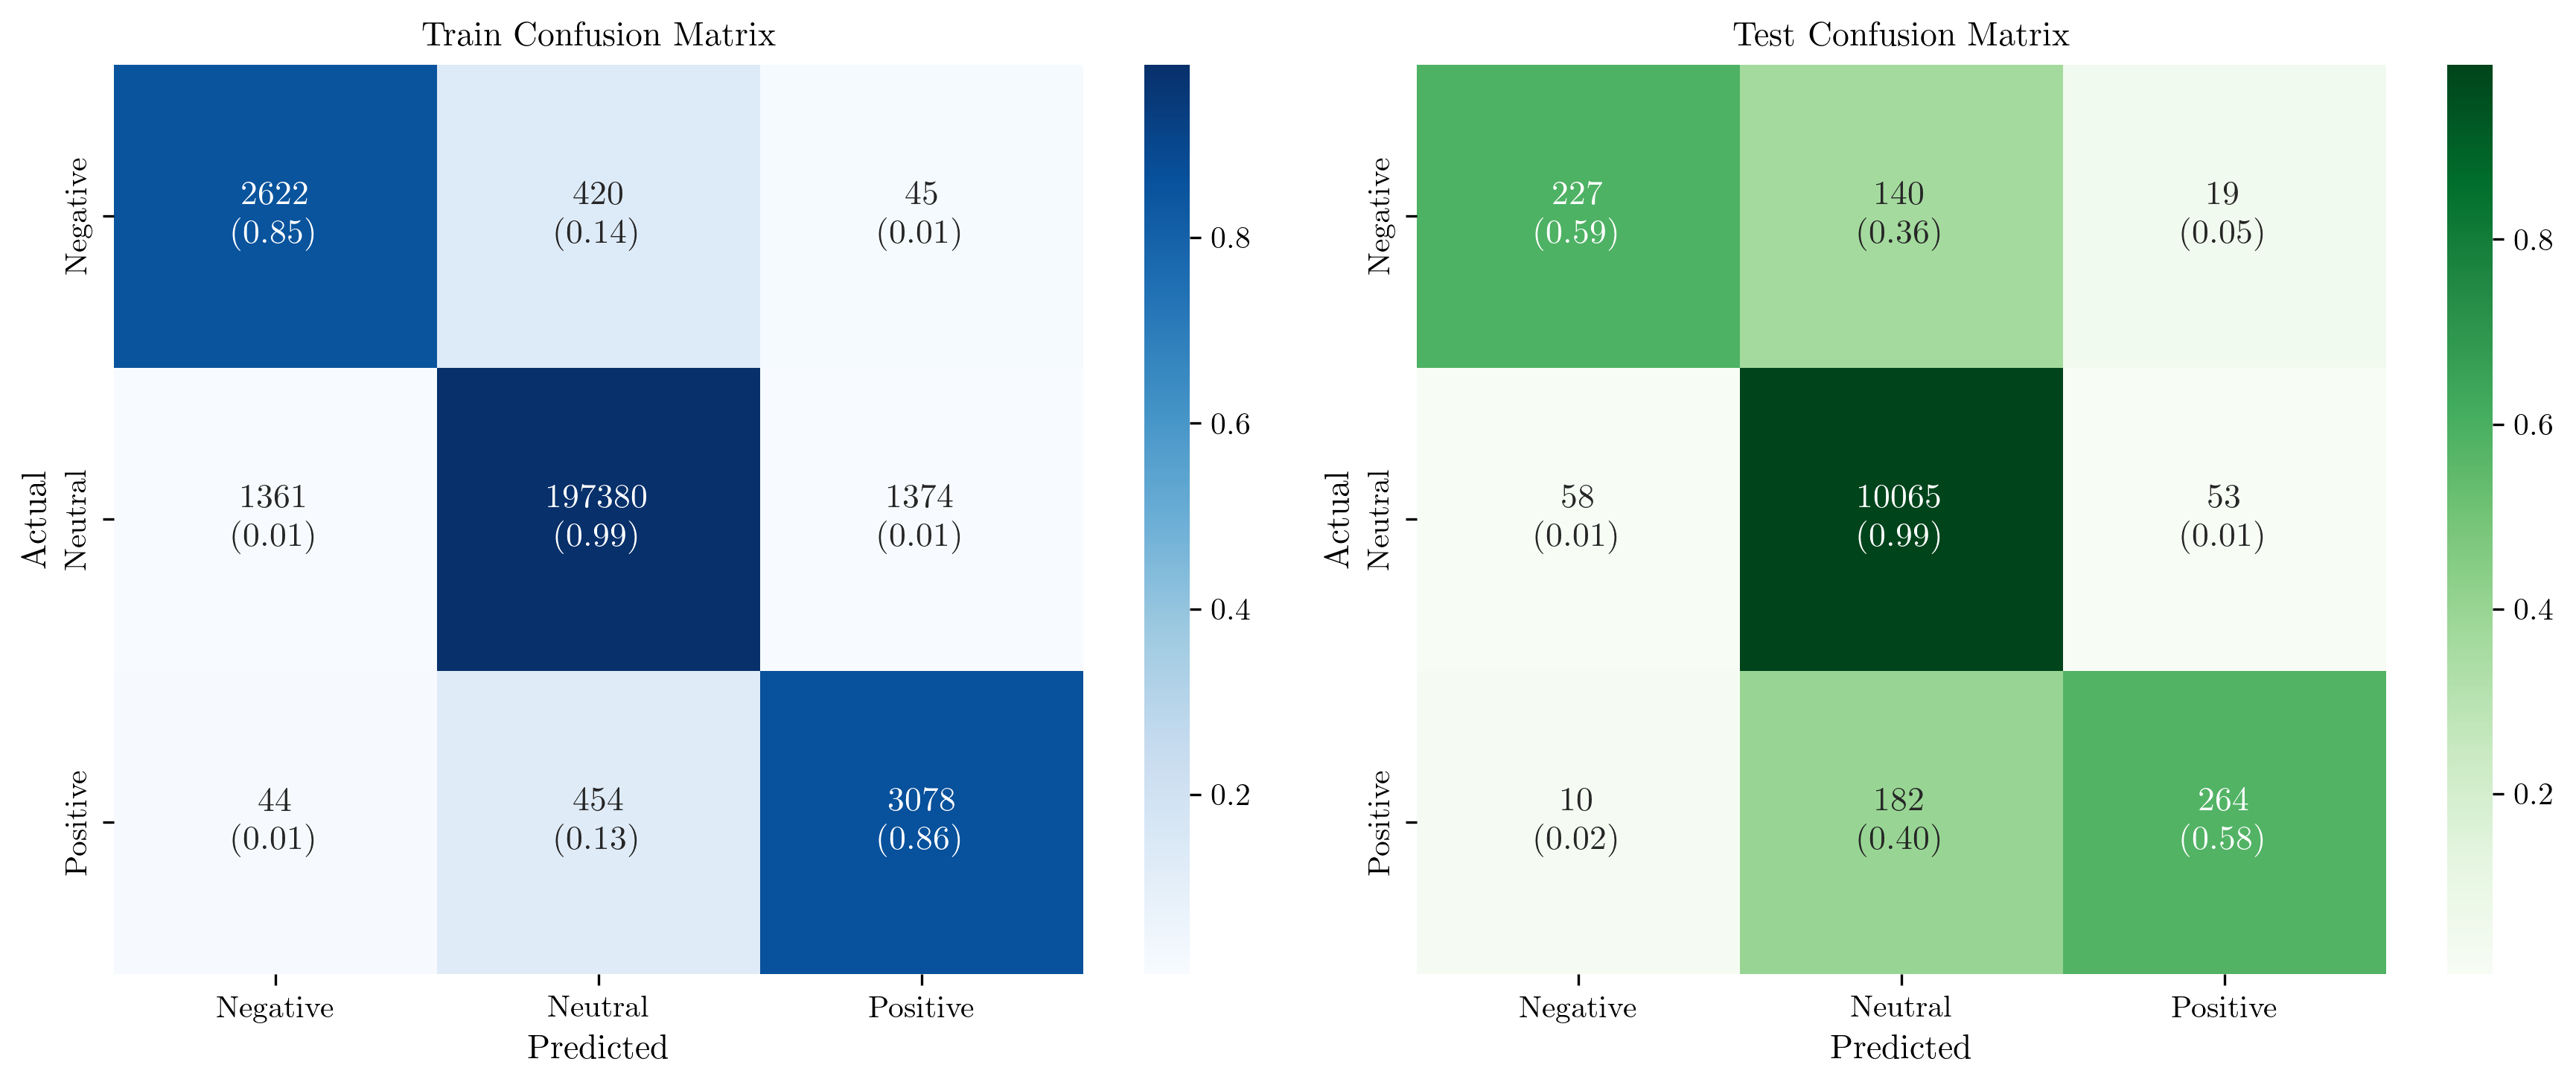
\includegraphics[width=1\textwidth]{figs/reddit_confusion_matrix.png}
        \caption{Confusion matrices for multi-sector sentiment classification of Reddit threads, with the training set shown on the left and the held-out test set on the right.}
    \label{fig:reddit_confusion_matrix}
\end{figure}

Table~\ref{tab:reddit_macro_f1_sector} reports the macro-F1 score per sector on the held-out test set. Performance varies substantially across sectors, ranging from $0.87$ for Energy down to $0.39$ for Consumer Staples. Sectors where synthetic data constituted a large share of the training set, notably Consumer Staples, Utilities, and Communication Services, tend to score lower, likely because the distribution of generated posts does not fully replicate the stylistic and topical variability of real Reddit threads. In addition, these sectors are genuinely less discussed in retail investor communities, meaning the model has fewer authentic signals to learn from and is more prone to defaulting to neutral predictions for the rare positive or negative cases in the test set.

\begin{table}[ht]
\centering
\caption{Macro-F1 score per sector for Reddit multi-sector sentiment classification on the held-out test set.}
\label{tab:reddit_macro_f1_sector}
\renewcommand{\arraystretch}{1.2}
\begin{tabular}{|l|c|c|}
\hline
\textbf{Sector} & \textbf{Macro-F1} & \textbf{Support} \\
\hline
Energy & 0.87 & 1045 \\
Materials & 0.72 & 997 \\
Industrials & 0.74 & 916 \\
Consumer Discretionary & 0.76 & 896 \\
Consumer Staples & 0.39 & 1060 \\
Health Care & 0.84 & 1055 \\
Financials & 0.81 & 937 \\
Information Technology & 0.76 & 947 \\
Communication Services & 0.68 & 1041 \\
Utilities & 0.46 & 1086 \\
Real Estate & 0.78 & 1038 \\
\hline
\end{tabular}
\label{tab:macro_f1_sector}
\end{table}


